\documentclass[10pt,t,aspectratio=169]{beamer}
%\usetheme{Berkeley}
\usepackage{graphicx}
\usepackage{amsmath}
\usepackage[american]{circuitikz}

% Packages to plot functions
\usepackage{pgfplots}
\pgfplotsset{compat=newest}

\usepackage{multicol}
\usepackage{multirow}
\usepackage{textcomp} % to use \textmu
\usepackage[absolute,overlay]{textpos} % to place floating text boxes with \begin{textblock*}{width}(x,y)
\usepackage{tcolorbox}
\usepackage{colortbl} % allows coloring cells of a table with \cellcolor{blue!25}

\title{Clase 2}
\subtitle{Semiconductores extrínsecos}
\author{Dr.-Ing. Juan José Montero Rodríguez}
\subject{Elementos Activos}
\institute{Escuela de Ingeniería Electrónica}
\date{Semestre II-2023}
\titlegraphic{
\includegraphics[height=12mm]{figures/logoTEC.pdf}}


\begin{document}

\begin{frame}[t]
\titlepage
\end{frame}


\begin{frame}[t]
  \frametitle{Dopado en Materiales Extrínsecos}

  \textbf{Dopado:} Introducción de impurezas (átomos) substitucionales en un material \textit{intrínseco} (puro) para modificar su conductividad eléctrica.

  \begin{figure}[H]
    \centering
    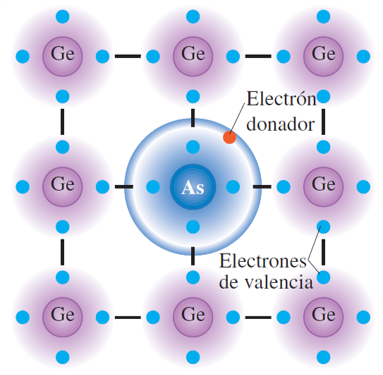
\includegraphics[width=5cm]{./figures/dopado1.png}
    \hspace{1cm}
    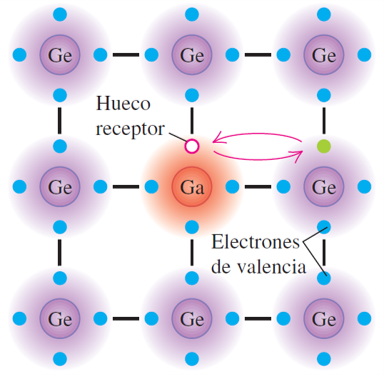
\includegraphics[width=5cm]{./figures/dopado2.png}
  \end{figure}
  
  \centering
  Los materiales dopados se conocen como materiales \textit{extrínsecos}
\end{frame}


\begin{frame}[t]
  \frametitle{Portadores Mayoritarios y Minoritarios}

  \begin{itemize}
    \item Existen dos portadores de carga en semiconductores:
    \begin{itemize}
      \item Electrones
      \item Huecos
    \end{itemize}
    \vspace{3mm}
    \item En un material extrínseco, se distingue entre portadores mayoritarios y minoritarios con base en la concentración de portadores.
    \vspace{3mm}
    \item \textbf{Portadores mayoritarios:} portadores presentes en mayor número en el semiconductor.
    \begin{itemize}
      \item Huecos en semiconductor P
      \item Electrones en semiconductor N
    \end{itemize}
    \vspace{3mm}
    \item \textbf{Portadores minoritarios:} portadores presentes en menor número en el semiconductor.
    \begin{itemize}
      \item Electrones en semiconductor P
      \item Huecos en semiconductor N
    \end{itemize}
  \end{itemize}
\end{frame}


\begin{frame}[t]
  \frametitle{Resumen de Definiciones}

  \begin{itemize}
    \item \textbf{Dopantes:} átomos de impureza específicos que se añaden a los semiconductores en dosis controladas, con la intención deliberada de incrementar las concentraciones de electrones o de huecos.
    \item \textbf{Semiconductor intrínseco:} semiconductor no dopado consistente en material semiconductor extremadamente puro, que contiene cantidades insignificantes de átomos de impureza; un semiconductor cuyas propiedades son inherentes al mismo.
    \item \textbf{Semiconductor extrínseco:} semiconductor dopado; un semiconductor cuyas propiedades están controladas por los átomos de impureza añadidos.
    \item \textbf{Donador:} átomo de impureza que incrementa la concentración de electrones; dopante tipo n.
    \item \textbf{Aceptor:} átomo de impureza que incrementa la concentración de huecos; dopante tipo p.
    \item \textbf{Material tipo n:} material dopado con donadores; un semiconductor que contiene más electrones que huecos.
    \item \textbf{Material tipo p:} material dopado con aceptores; un semiconductor que contiene más huecos que electrones.
  \end{itemize}
\end{frame}


\begin{frame}[t]
  \frametitle{Dopado}

  \begin{itemize}
    \item Donadores: 5 electrones de valencia  (As, P, Sb) = semiconductor de tipo N.
    \item Aceptores: 3 electrones de valencia (B, In) = semiconductor de tipo P.   
  \end{itemize}

  \begin{figure}[H]
    \centering
    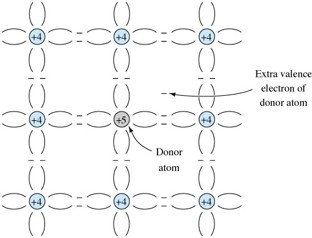
\includegraphics[width=6cm]{./figures/dopado3.jpg}
    \hspace{1cm}
    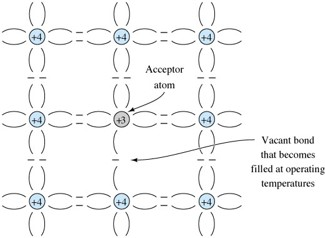
\includegraphics[width=6cm]{./figures/dopado4.jpg}
  \end{figure}

  \centering
  \textbf{El dopado NO ALTERA la neutralidad eléctrica del material}
\end{frame}


\begin{frame}[t]
  \frametitle{Dopantes Comunes para Silicio}

  \begin{columns}
    \begin{column}{0.5\textwidth}
      Los dopantes más comunes para Silicio se muestran en la tabla:
      \begin{itemize}
        \item Átomos de la columna V aportan electrones.
        \item Átomos de la columna III aportan huecos.
      \end{itemize}

      \begin{table}[H]
        \centering
        \begin{tabular}{cc}
          \hline \textbf{Donadores} & \textbf{Aceptores} \\
          \hline P & B \\
          As & Ga \\
          Sb & In \\
          & Al \\
          \hline
        \end{tabular}
      \end{table}

      \centering El material permanece eléctricamente neutro porque el número de electrones es igual al número de protones para ambos casos.

      \vspace{4mm}
      \textbf{No existe carga eléctrica en el material}
    \end{column}
    \begin{column}{0.5\textwidth}
      \centering
      Los átomos dopantes tienen a su portador enlazado al núcleo, requieren de cierta energía para que el portador sea liberado al material.

      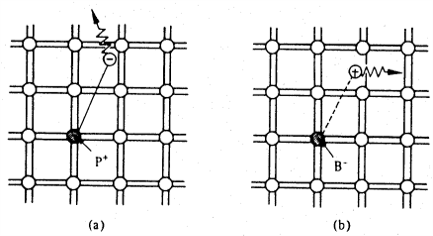
\includegraphics[width=6cm]{./figures/dopado5.png}

      \begin{table}[H]
        \centering
        \begin{tabular}{cc}
          \hline \textbf{Material} & \textbf{Energía Ionización}\\
          \hline Fósforo & 0.045 eV \\
          Arsénico & 0.050 eV \\
          Boro & 0.045 eV \\
          Aluminio & 0.060 eV \\
          \hline
        \end{tabular}
      \end{table}
    \end{column}
  \end{columns}
\end{frame}


\begin{frame}[t]
  \frametitle{Activación (Ionización) de los Dopantes con la Temperatura}

  \centering
  Semiconductor N: se introducen estados energéticos cerca de la banda $E_C$

  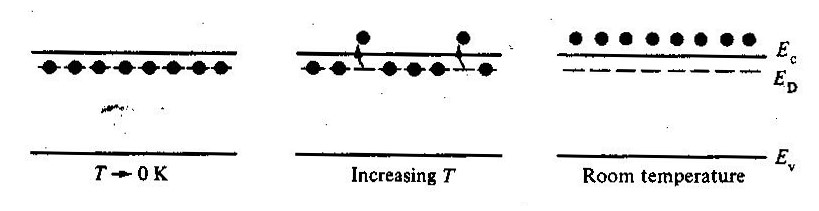
\includegraphics[width=12cm]{./figures/ionizacion1.jpg}

  Semiconductor P: se introducen estados energéticos cerca de la banda $E_V$

  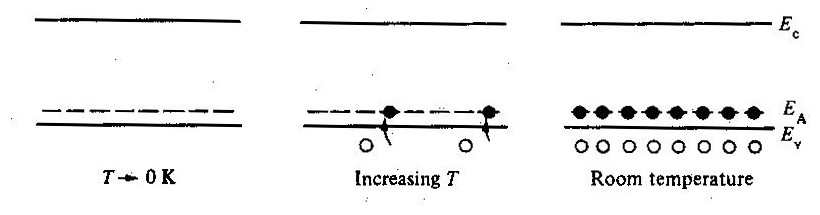
\includegraphics[width=12cm]{./figures/ionizacion2.jpg}
\end{frame}


\begin{frame}
  \frametitle{Ley de Acción de Masas}

  En un semiconductor no degenerado en equilibrio:

  \begin{columns}
    \begin{column}{0.3\textwidth}
      \[ n_i^2 = n\times{}p \]
    \end{column}
    \begin{column}{0.7\textwidth}
      \begin{itemize}
        \item ni : concentración intrínseca de portadores de carga [cm\textsuperscript{-3}]
        \item n: concentración de electrones libres [cm\textsuperscript{-3}]
        \item p: concentración de huecos [cm\textsuperscript{-3}]
      \end{itemize}
    \end{column}
  \end{columns}

  \vspace{5mm}
  \[ n_i \approx 1\times{}10^{10}\ cm^{-3} \]
  
  \vspace{5mm}
  Lo anterior implica que:

  \begin{itemize}
    \item Si el material es intrínseco, se observa que $n=p=n_i$.
    \item Si la concentración de electrones aumenta con el dopado (donadores), la concentración de huecos disminuye.
    \item Si la concentración de huecos aumenta con el dopado (aceptores), la concentración de electrones disminuye.
  \end{itemize}
\end{frame}


\begin{frame}[t]
  \frametitle{Concentración de Portadores de Carga}

  \begin{columns}
    \begin{column}{0.5\textwidth}
      Para un material tipo P:

      \[ p \approx N_A \]

      \[ n \approx \dfrac{n_i^2}{N_A} \]

      \begin{itemize}
        \item $N_A$: Concentración de átomos dopantes aceptores por cm\textsuperscript{3}
        \item $p$: Concentración de huecos por cm\textsuperscript{3}
        \item $n$: Concentración de electrones por cm\textsuperscript{3}
      \end{itemize}
    \end{column}
    \begin{column}{0.5\textwidth}
      Para un material tipo N:

      \[ n \approx N_D \]
    
      \[ p \approx \dfrac{n_i^2}{N_D} \]

      \begin{itemize}
        \item $N_D$: Concentración de átomos dopantes donadores por cm\textsuperscript{3}
        \item $p$: Concentración de huecos por cm\textsuperscript{3}
        \item $n$: Concentración de electrones por cm\textsuperscript{3}
      \end{itemize}
    \end{column}
  \end{columns}

  \vspace{5mm}
  Los cálculos anteriores son válidos para \textbf{semiconductores no degenerados}, en \textbf{equilibrio térmico} y con \textbf{temperatura constante}, cuando existe un único tipo de átomo dopante.
\end{frame}


\begin{frame}[t]
  \frametitle{Efecto del Dopado en el Nivel de Fermi}

  \begin{columns}
    \begin{column}{0.4\textwidth}
      \[ E_i - E_F = kT \ln \dfrac{N_A}{n_i} \]
      
      \vspace{5mm}
      \[ E_F - E_i = kT \ln \dfrac{N_D}{n_i} \]
    \end{column}
    \begin{column}{0.6\textwidth}
      \centering
      Diferencia entre nivel de Fermi intrínseco y extrínseco del semiconductor P

      \vspace{5mm}
      Diferencia entre nivel de Fermi intrínseco y extrínseco del semiconductor N      
    \end{column}
  \end{columns}

  \vspace{5mm}
  La concentración de portadores de carga y el nivel de Fermi están relacionados como sigue:

  \vspace{5mm}
  \begin{columns}
    \begin{column}{0.5\textwidth}
      \[ n = n_i \cdot e^{\dfrac{E_F - E_i}{kT}} \]
    \end{column}
    \begin{column}{0.5\textwidth}
      \[ p = n_i \cdot e^{\dfrac{E_i - E_F}{kT}} \]
    \end{column}
  \end{columns}
\end{frame}


\begin{frame}[t]
  \frametitle{Efecto del Dopado en el Nivel de Fermi}

  En un semiconductor N, el nivel de Fermi se acerca a la banda de conducción

  \begin{figure}[H]
    \centering
    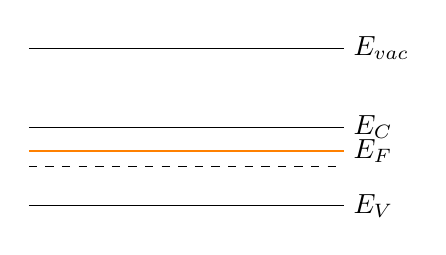
\begin{tikzpicture}
      \draw (0,0) -- (4,0);
      \draw (4,0) node[anchor=west]{$E_{vac}$};
      \draw (0,-1) -- (4,-1);
      \draw (4,-1) node[anchor=west]{$E_{C}$};
      \draw [dashed] (0,-1.5) -- (4,-1.5);
      %\draw (4,-1.5) node[anchor=west]{$E_{i}$};
      \draw (0,-2) -- (4,-2);
      \draw (4,-2) node[anchor=west]{$E_{V}$};
      \draw [thick,orange] (0,-1.3) -- (4,-1.3);
      \draw (4,-1.3) node[anchor=west]{$E_{F}$};
    \end{tikzpicture}
  \end{figure}

  En un semiconductor P, el nivel de Fermi se acerca a la banda de valencia

  \begin{figure}[H]
    \centering
    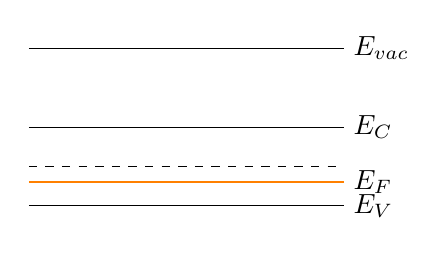
\begin{tikzpicture}
      \draw (0,0) -- (4,0);
      \draw (4,0) node[anchor=west]{$E_{vac}$};
      \draw (0,-1) -- (4,-1);
      \draw (4,-1) node[anchor=west]{$E_{C}$};
      \draw [dashed] (0,-1.5) -- (4,-1.5);
      %\draw (4,-1.5) node[anchor=west]{$E_{i}$};
      \draw (0,-2) -- (4,-2);
      \draw (4,-2) node[anchor=west]{$E_{V}$};
      \draw [thick,orange] (0,-1.7) -- (4,-1.7);
      \draw (4,-1.7) node[anchor=west]{$E_{F}$};
    \end{tikzpicture}
  \end{figure}
\end{frame}


\begin{frame}[t]
  \frametitle{Semiconductores Degenerados}

  Semiconductor N degenerado: nivel de Fermi está a $<3kT$ de la banda $E_C$


  \begin{figure}[H]
    \centering
    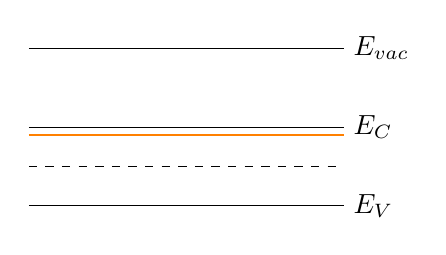
\begin{tikzpicture}
      \draw (0,0) -- (4,0);
      \draw (4,0) node[anchor=west]{$E_{vac}$};
      \draw (0,-1) -- (4,-1);
      \draw (4,-1) node[anchor=west]{$E_{C}$};
      \draw [dashed] (0,-1.5) -- (4,-1.5);
      %\draw (4,-1.5) node[anchor=west]{$E_{i}$};
      \draw (0,-2) -- (4,-2);
      \draw (4,-2) node[anchor=west]{$E_{V}$};
      \draw [thick,orange] (0,-1.1) -- (4,-1.1);
      %\draw (4,-1.3) node[anchor=west]{$E_{F}$};
    \end{tikzpicture}
  \end{figure}

  Semiconductor P degenerado: nivel de Fermi está a $<3kT$ de la banda $E_V$

  \begin{figure}[H]
    \centering
    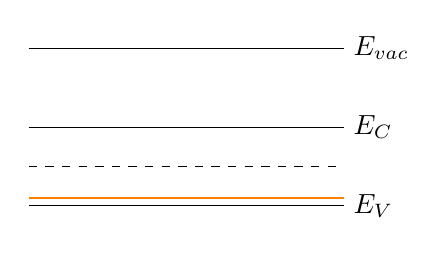
\begin{tikzpicture}
      \draw (0,0) -- (4,0);
      \draw (4,0) node[anchor=west]{$E_{vac}$};
      \draw (0,-1) -- (4,-1);
      \draw (4,-1) node[anchor=west]{$E_{C}$};
      \draw [dashed] (0,-1.5) -- (4,-1.5);
      %\draw (4,-1.5) node[anchor=west]{$E_{i}$};
      \draw (0,-2) -- (4,-2);
      \draw (4,-2) node[anchor=west]{$E_{V}$};
      \draw [thick,orange] (0,-1.9) -- (4,-1.9);
      %\draw (4,-1.7) node[anchor=west]{$E_{F}$};
    \end{tikzpicture}
  \end{figure}
\end{frame}


\begin{frame}[t]
  \frametitle{Principio de Neutralidad de Carga}

  En un semiconductor en equilibrio térmico, uniformemente dopado y bajo condiciones de dopado no degenerado, se cumple que

  \[ qp - qn + qN_D^+ - qN_A^- = 0 \]

  Lo que es equivalente a

  \[ p - n + N_D^+ - N_A^- = 0 \]

Donde, por definición,

\begin{itemize}
  \item $N_D^+$: número de impurezas donadoras ionizadas/cm\textsuperscript{3}
  \item $N_A^-$: número de impurezas aceptoras ionizadas/cm\textsuperscript{3}
\end{itemize}

\vspace{3mm}
A temperatura ambiente, todas las impurezas están ionizadas, por lo que:

\[ p - n + N_D - N_A = 0 \]
\end{frame}


\begin{frame}[t]
  \frametitle{Balance de Cargas y Compensación}

  \begin{columns}
    \begin{column}{0.6\textwidth}
      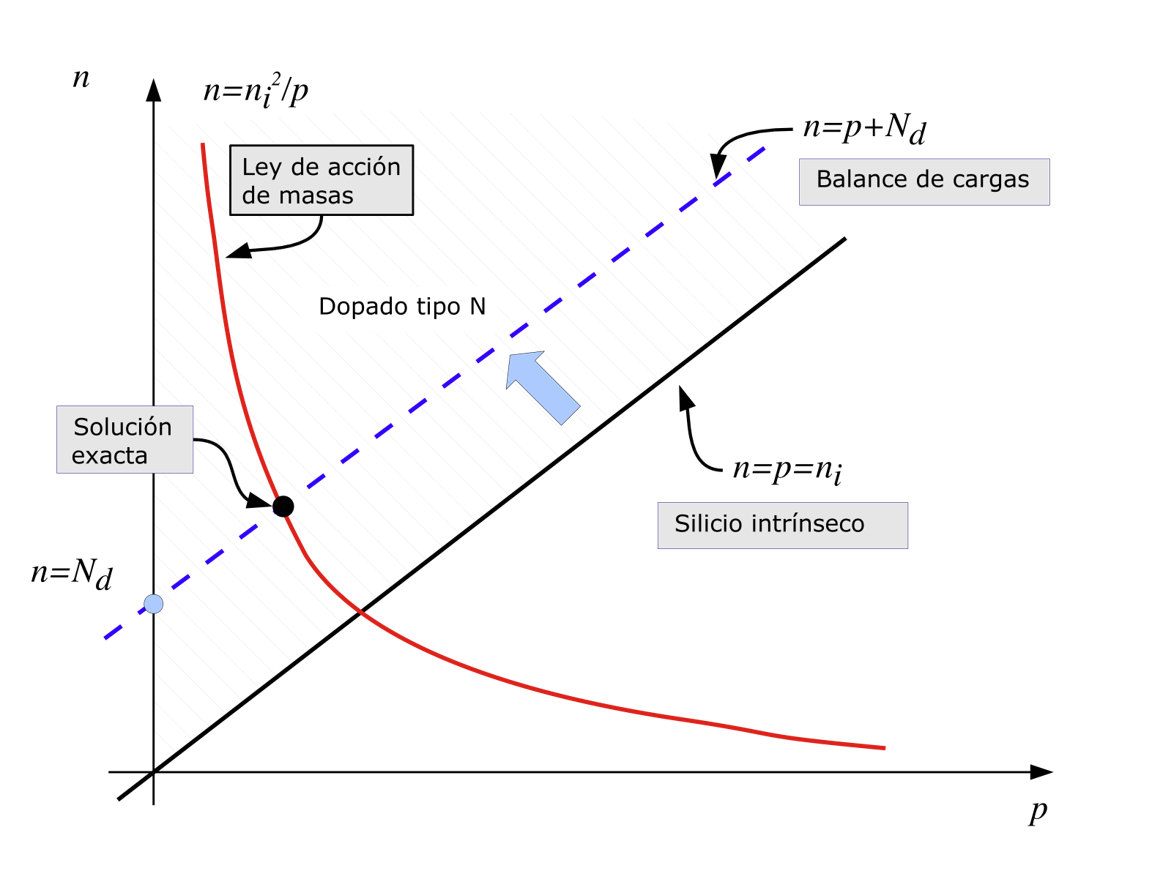
\includegraphics[width=9.5cm]{./figures/curvanvsp.png}      
    \end{column}
    \begin{column}{0.4\textwidth}
      
      \begin{itemize}
        \item En la figura se observa la ley de acción de masas:
        \[ n = n_i^2/p \]
        \item Si el material es intrínseco, se obtiene la identidad $n=p=n_i$.
        \item Al dopar el material con donadores $N_D$, el balance de cargas da:
      \end{itemize}
      %
      \[ p - n + N_D - N_A = 0 \]
      %
      \[ p - n + N_D - 0 = 0 \]
      %
      \[ n = p + N_D \]
      %
      Esto corresponde a desplazar la identidad hacia arriba.
    \end{column}
  \end{columns}

\end{frame}

\begin{frame}[t]
  \frametitle{Balance de Cargas y Compensación}

  \begin{columns}
    \begin{column}{0.6\textwidth}
      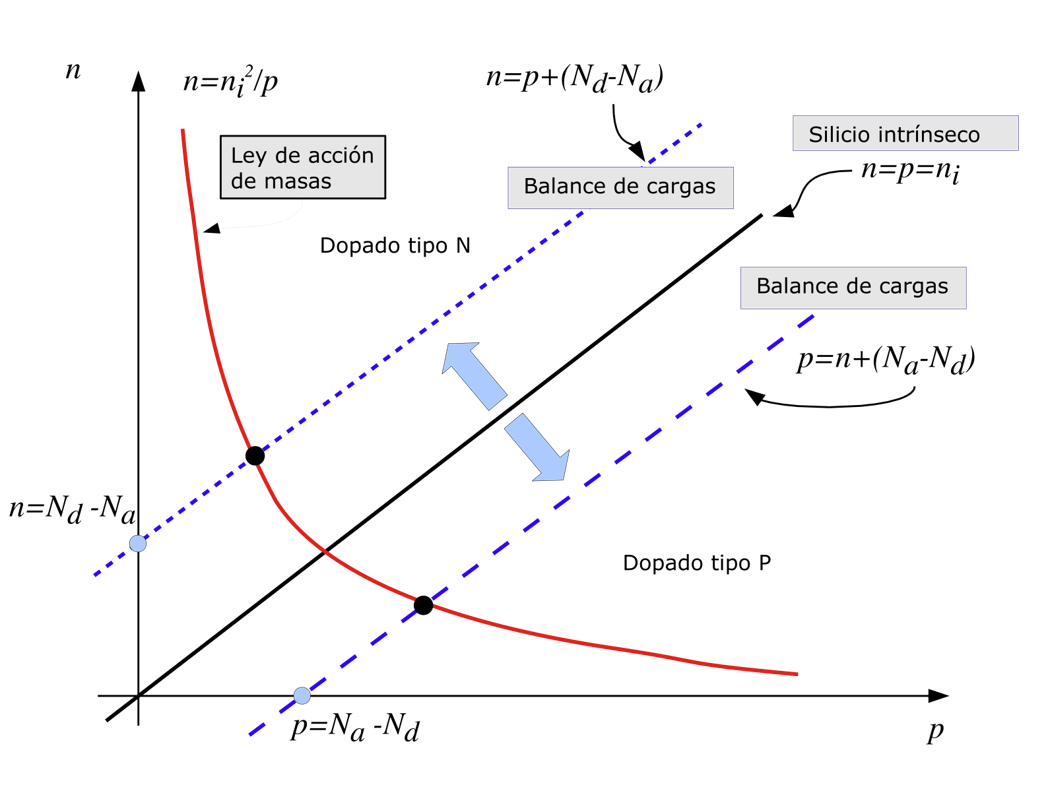
\includegraphics[width=9.5cm]{./figures/curvanvsp2.png}      
    \end{column}
    \begin{column}{0.4\textwidth}
      \begin{itemize}
        \item Si a un material previamente dopado con $N_D$ se dopa ahora además con $N_A$:
      \end{itemize}
      %
      \[ p - n + N_D - N_A = 0 \]
      %
      \[ n \approx N_D - N_A \]
      %
      \begin{itemize}
        \item El dopado efectivo es igual a la diferencia de ambos dopados.
        \item Los aceptores ``cancelan'' a los donadores.
        \item Se debe revisar cuál es el dopado más fuerte:
        \begin{itemize}
          \item $N_D-N_A>0 \Rightarrow$ dopado N
          \item $N_A-N_D>0 \Rightarrow$ dopado P
        \end{itemize}
      \end{itemize}
    \end{column}
  \end{columns}
\end{frame}


\begin{frame}[t]
  \frametitle{Efecto de la Temperatura en Semiconductores Extrínsecos}

  Temperatura afecta el comportamiento de semiconductores:

  \begin{itemize}
    \item Bajas temperaturas: energía térmica insuficiente para ionizar todos los átomos de impurezas.
    \begin{itemize}
      \item Concentración de portadores mayoritarios es menor que concentración de dopado.
    \end{itemize}
    \item Temperaturas medias: energía térmica es suficiente para ionizar todos los átomos de impurezas.
    \item Altas temperaturas: El nivel de Fermi se acerca al nivel de Fermi intrínseco.
    \begin{itemize}
      \item Material se comporta como semiconductor intrínseco.
    \end{itemize}
  \end{itemize}
  
  Resumen:

  \begin{itemize}
    \item $n_i$ en un semiconductor intrínseco aumenta con $T$
    \item Conductividad aumenta con T
  \end{itemize}
\end{frame}


\begin{frame}[t]
  \frametitle{Efecto de la Temperatura en Semiconductores Extrínsecos}

  \begin{columns}
    \begin{column}{0.5\textwidth}
      \centering
      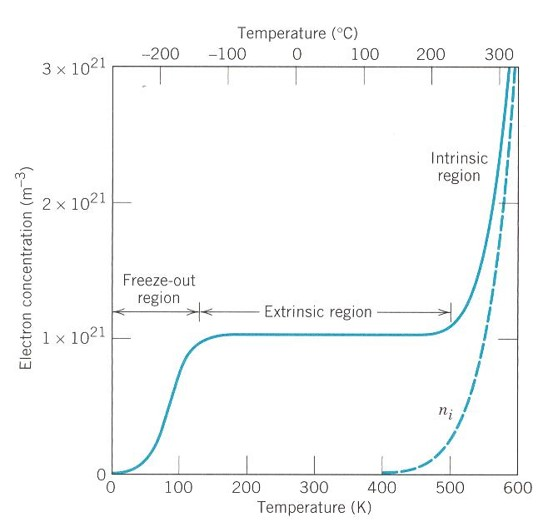
\includegraphics[height=7cm]{./figures/temp1.jpg}
    \end{column}
    \begin{column}{0.5\textwidth}
      \centering
      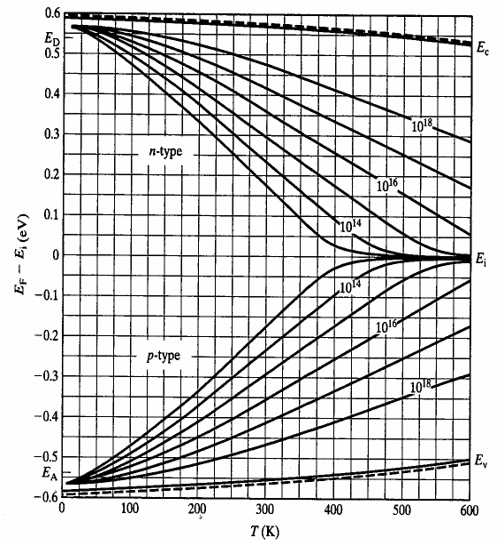
\includegraphics[height=7cm]{./figures/temp2.png}
    \end{column}
  \end{columns}
\end{frame}


\begin{frame}[t]
  \frametitle{Ejemplo: Ley de Acción de Masas}

  Para fabricar circuitos integrados, se dopa un oblea de silicio con una concentración de aceptores $N_A=10^{15}\ cm^{-3}$.
 
  \begin{itemize}
    \item ¿Cuál es la concentración de portadores mayoritarios en la oblea?
    \[ p \approx N_A = 10^{15}\ huecos/cm^3 \]
    \item ¿Cuál es la concentración de portadores minoritarios en la oblea?
    \[ n \approx \dfrac{n_i^2}{N_A} = \dfrac{(10^{10})^2}{10^{15}} = 10^5\ electrones/cm^3 \]
    \item Si la concentración de huecos se incrementa a $N_A=10^{16}\ cm^{-3}$ por medio de dopado adicional, ¿Cuál es la nueva concentración de portadores minoritarios en la oblea?
    \[ n \approx \dfrac{n_i^2}{N_A} = \dfrac{(10^{10})^2}{10^{16}} = 10^4\ electrones/cm^3 \]
  \end{itemize}
\end{frame}


\begin{frame}[t]
  \frametitle{Ejemplo: Dopado y Compensación}

  \begin{itemize}
    \item Una oblea de silicio está dopada con boro, con una concentración de portadores de $10^{15}\ cm^{-3}$. Para este material, determine la posición del nivel de Fermi con respecto al nivel de Fermi intrínseco.
    \item La oblea del caso anterior se dopa ahora con arsénico, donde se implanta una concentración de átomos de arsénico de $2.1\times{}10^{15}\ cm^{-3}$. Bajo estas condiciones indique:
    \begin{itemize}
      \item El nivel de dopado efectivo resultante.
      \item La concentración de portadores (n y p) resultante.
      \item La nueva posición del nivel de Fermi con respecto a Ei.
    \end{itemize}
    \item Suponiendo que se hace una segunda implantación iónica con arsénico, donde se quiere aumentar al máximo la conductividad de la muestra, calcule ¿cuál es la concentración máxima de átomos donadores permitida para que el material siga siendo no degenerado?
  \end{itemize}

\end{frame}

\begin{frame}{Lecturas recomendadas}
    
\end{frame}

\end{document}
